\documentclass[11pt]{article}

%imports
\usepackage[utf8]{inputenc}
\usepackage[T1]{fontenc}
\usepackage{amsmath}
\usepackage{amsfonts}
\usepackage{amssymb}
\usepackage{footnote}
\usepackage{url}
\usepackage{natbib}

%images and image path
\usepackage{graphicx}
\graphicspath{ {./images/} }

%custom commands
\newcommand{\N}{\mathcal{N}}
\newcommand{\num}{\text{num}}
\newcommand{\obs}{\text{obs}}
\newcommand{\D}{\mathfrak{D}}
\newcommand{\Ro}{\mathcal{R}_0}

\DeclareRobustCommand{\firstsecond}[2]{#1}

%margins
\usepackage[letterpaper, total={6.5in, 9.5in}]{geometry}

%opening
\title{Reaction-diffusion spatial modeling of COVID-19 in Chicago}
\author{Trent Gerew}

\begin{document}

\maketitle

\begin{abstract}
	We examine an application of the Law of Mass Action to model the outbreak of COVID-19 in Chicago.
	We begin with a zero-dimension (ODE) compartmental epidemiological model consisting of Susceptible, Infected, and Removed populations (SIR model).
	We then develop a spatially distributed version of the model in the form of reaction-diffusion equations (PDE).
\end{abstract}

\section{Introduction and Similar Work}

\section{ODE and PDE Model Setup}
We begin by explaining the ODE model which is simply obtained from the full PDE model by removing the diffusion terms in the reaction-diffusion equations.

We start with a population of \textit{susceptibles} ($S$), which may become \textit{infected} ($I$) upon the emergence of the virus within the population.
Infected individuals can interact with the susceptibles at rate $\beta$ to draw new members into the group $I$ of individuals infected by the virus.
We note that the transmission rate $\beta$ incorporates the total population size (ODE model) or the total population density (PDE model).
A fraction of the infected population recover or die at a rate $\gamma$, giving rise to the \textit{removed} ($R$) population.

These parameters specify the ODE process.
They represent processes that occur in a ``well mixed'' situation when no spatial dependence is assigned,
or processes that happen locally at every point in space for the PDE's.
We discuss parameter selection in the next section.

\begin{figure}[h]
	\centering
	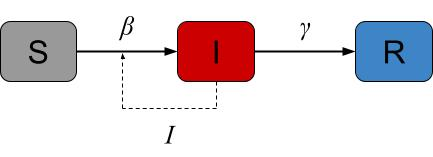
\includegraphics[width=0.5\textwidth]{sir_schematic}
	\caption{Schematic diagram of the SIR model. The dashed line denotes the interaction of the infectious population with the susceptible population that leads to infection.}
	\label{fig:schematic}
\end{figure}

The population model at the PDE level is an autonomous diffusion with a source:
\begin{align}
	S_t	&=	\Delta (\D_s \Delta S) - \beta SI,	\\
	I_t	&=	\Delta (\D_I \Delta I) + \beta SI - \gamma I,	\\
	R_t	&=	\gamma I.
\end{align}
In principle the $R$ population can have a diffusion, but since we assume this population has immunity we assign $\D_R = 0$.

As in \cite{Kevrekidis_2021}, we have not incorporated any functional forms for directional spreading at the PDE level.
In principle, these terms can represent ``daily practices'' (work commutes, etc.), as well as longer temporal or spatial scales (major thoroughfare traffic, etc.).
We simply allow diffusion to perform the relevant spreading.
Arriving infected individuals are assumed to form local hotspots within the susceptible population.
This initial seeding roughly approximates long-range transportation.

The next step is to identify the parameters at the ODE level.
To do this, we use a nonlinear optimization algorithm.
We determine the optimal parameters by minimizing the Euclidean distance between the time series generated by the model ($\num$) and the corresponding observed ($\obs$) time series,
\begin{equation}
	\N = \sum_i \left( \left| \log(C_\num (t_i)) - \log(C_\obs (t_i)) \right|^2 + \left| \log(R_\num (t_i)) - \log(R_\obs (t_i)) \right|^2 \right)
\end{equation}
where the index $i$ identifies a point in the time series.
The parameters are optimized to reproduce the reported total number of infected cases $C(t) = I(t) + R(t)$, and the total number of removed $R(t)$.

Since the transition rate $\gamma$ is an ``individual'' parameter, and thus acts ``on average'', we preserve the same value at the PDE level as at the ODE level.
The transmission rate $\beta$ is more complicated, since at the PDE level the quantities $S$, $I$, and $R$ are densities rather than populations,
which integrate over the spatial surface to the true population of each category.

\subsection{ODE Dynamics}
Here we briefly discuss some dynamics of the ODE system.
Note that for the simply SIR model as we have here, $R$ is completely determined when $S$ and $I$ are known, so we need only consider
\begin{align*}
	S_t	&=	- \tilde{\beta} SI, \\
	I_t	&=	\tilde{\beta} SI - \gamma I,
\end{align*}
where $\tilde{\beta} = \beta / N$.

Immediately we see there are infinitely many non-isolated fixed points of the form $(S,0)$.
Linearizing, we get
\begin{equation*}
	\mathbf{A}_{(S,0)} = \begin{bmatrix} 0 & - \tilde{\beta} S \\ 0 & \beta S - \gamma \end{bmatrix}.
\end{equation*}
Thus, as seen in Figure \ref{fig:localdyn}, for $S < \frac{\gamma}{\tilde{\beta}}$ the nodes are stable, and for $S > \frac{\gamma}{\tilde{\beta}}$ they are unstable.
\begin{figure}[h]
	\centering
	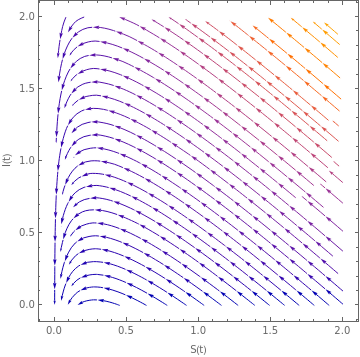
\includegraphics[width=0.25\textwidth]{local_dynamics}
	\caption{Stream plot for the local ODE dynamics. Note the transcritical bifurcation around $S_0 = 0.4$.}
	\label{fig:localdyn}
\end{figure}
We can then conclude that an epidemic will occur only if $S_0 = S(t=0) > \frac{\gamma}{\tilde{\beta}}$ \cite{Wang_SIR}.
Hence, a transcritical bifurcation occurs at $\Ro = \tilde{\beta} S_0 / \gamma$, which is known as the \textit{basic reproduction number},. and is used to estimate how the epidemic developed initially.

Note that the SIR model can be viewed as a generalized chemical reaction
\begin{align*}
	S + I	&\longrightarrow	2 I, \\
	I		&\longrightarrow	R.
\end{align*}
However, these two reactions are not reversible, so we are not able to write the energy-dissipation law for the SIR model \cite{Forster_2013, Wang_2020}.
Indeed, taking $\frac{I_t}{S_t} = - 1 + \frac{\gamma}{\tilde{\beta} S}$ and solving this differential equation gives $I = - S + \frac{\gamma}{\tilde{\beta}} \ln(S) + C$.
Thus,
\begin{equation}
	E(S,I) = S + I - \frac{\gamma}{\tilde{\beta}} \ln(S)
\end{equation}
is a conserved quantity for the system.

\section{Results}
\subsection{ODE Model}
We begin by discussing the zero-dimensional model for Chicago.
Data for the progression of the pandemic in Chicago were obtained from the Chicago Data Portal \cite{Chicago_2021}.

\begin{savenotes}
\begin{table}[h]
	\centering
	\caption{ODE parameters}
	\label{tab:parameters}
	\begin{tabular}{ c c c c }
		\hline
		\hline
			&	&	Optimal	&	Initial value \\
		\hline
		Population	&	$N$	&	2,695,598 \\
		Initial population	&	$I_0$	&	 \\
		Transmission rate, $S \rightarrow I$ [per day]	&	$\beta$\footnote{The transmission rate $\beta$ must be divided by $N$ when used in the ODE model.}	&	&	$c \in U[0,1]$ \\
		Transition rate, $I \rightarrow R$ [per day]	&	$\gamma$	&		&	$c \in U[0.25,0.75]$ \\
		Diffusivity, $S$ [km$^2$/day]	&	$\D_S$	&	10	&	\\
		Diffusivity, $I$ [km$^2$/day]	&	$\D_I$	&	100	&	\\
		\hline
		\hline
	\end{tabular}
\end{table}
\end{savenotes}


\bibliographystyle{abbrv}
\bibliography{chicago-spatial-covid-draft}

\end{document}
